\documentclass[tikz,border=3mm]{standalone}
\usepackage[siunitx]{circuitikz}
\usetikzlibrary{calc,positioning,arrows.meta}

\begin{document}

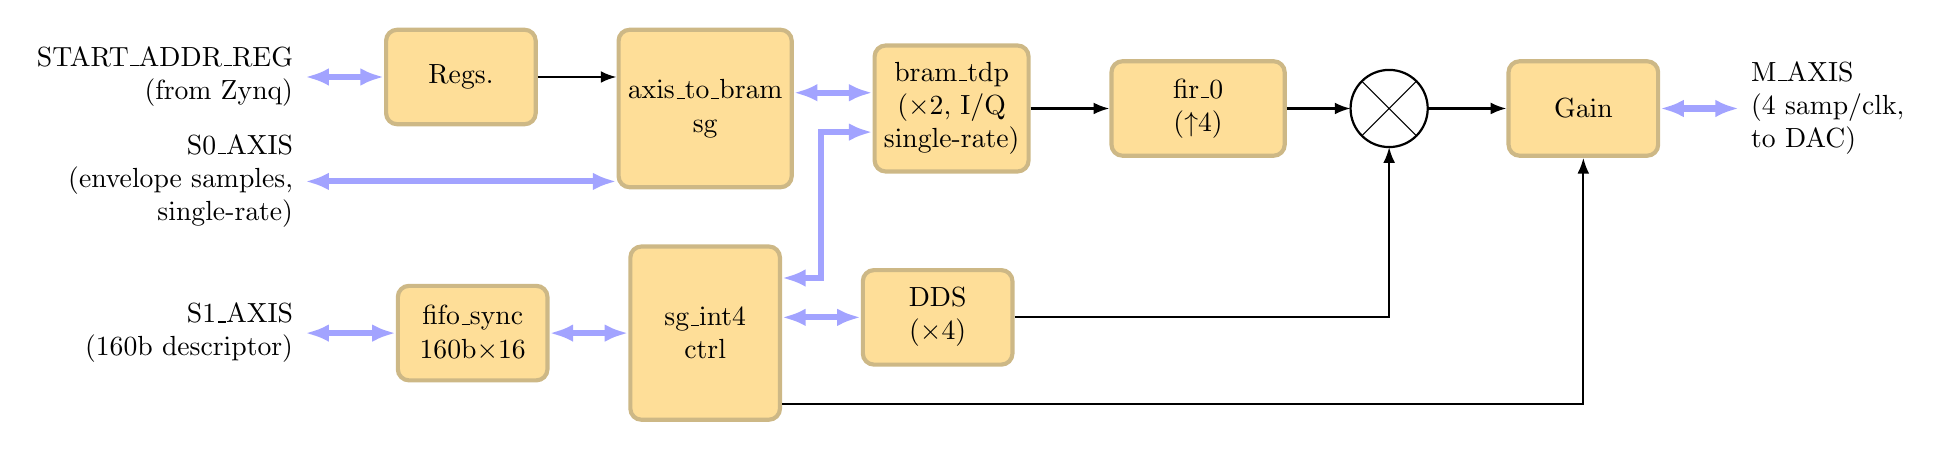
\begin{tikzpicture}
[box/.style={align=center, draw,rounded corners,minimum width=1.9cm,minimum height=1.2cm,draw={rgb,255:red,205; green,184; blue,134},fill={rgb,255:red,254; green,222; blue,152},line width=1.5pt},
arrow/.style={line width=2.2pt,draw={rgb,255:red,162; green,163; blue,255},{Latex[length=3mm]}-{Latex[length=3mm]}},
single arrow/.style={line width=0.8pt,-{Latex[length=2mm]}},
node distance=0.4cm]

% Data writer.
\node[box,minimum height=2cm] (data writer) {axis\_to\_bram\\ sg};

% Control.
\node[box,below=0.7cm of data writer,minimum height=2.2cm] (ctrl) {sg\_int4\\ ctrl};

% Memory (single-rate, real+imag).
\node[box,right=1cm of data writer,minimum height=1.6cm] (mem) {bram\_tdp\\ ($\times$2, I/Q\\ single-rate)};

% Interpolating FIR.
\node[box,right=1cm of mem,minimum width=2.2cm] (fir) {fir\_0\\($\uparrow$4)};

% DDS.
\coordinate (temp) at ($(ctrl.north east)+(1,-0.3)$);
\node[box,anchor=north west] (dds) at (temp) {DDS\\($\times$4)};

% Regs.
\coordinate (temp) at ($(data writer.north west)+(-1,0)$);
\node[box,anchor=north east] (axi regs) at (temp) {Regs.};

% Fifo.
\node[box,left=1cm of ctrl] (fifo) {fifo\_sync\\160b$\times$16};

% Mixer.
\coordinate (temp) at ($(fir.east)+(1.3,0)$);
\node[mixer] (mixer) at (temp) {};

% Gain.
\node[box,right=1cm of mixer] (gain) {Gain};

% s_axi (registers).
\draw[arrow] ($(axi regs.west)+(-1,0)$) coordinate (s axi in) node[anchor=east,align=right] {START\_ADDR\_REG\\(from Zynq)} -- (axi regs.west);

% s0_axis.
\draw[arrow] ($(s axi in |- axi regs.south)+(0,-0.7)$) coordinate (temp) node[anchor=east,align=right] {S0\_AXIS\\(envelope samples,\\ single-rate)} -- (temp -| data writer.west);

% s1_axis.
\draw[arrow] (s axi in |- fifo.west) coordinate (temp) node[anchor=east,align=right] {S1\_AXIS\\(160b descriptor)} -- (temp -| fifo.west);

% Regs -> data writer.
\draw[single arrow] (axi regs) -- (axi regs -| data writer.west);

% Data writer -> memory.
\draw[arrow] ($(data writer.east)+(0,0.2)$) coordinate (temp) -- (temp -| mem.west);

% Control -> dds.
\draw[arrow] (dds.west) -- (dds.west -| ctrl.east);

% Control -> memory (mem_addrb).
\draw[arrow] ($(ctrl.east)+(0,0.7)$) -- ++(0.5,0) |- ($(mem.west)+(0,-0.3)$);

% Control -> Fifo (fifo_rd_en).
\draw[arrow] (ctrl) -- (fifo);

% memory -> fir (x4 interpolation).
\draw[single arrow] (mem.east) -- (fir.west);

% fir -> mixer (envelope, now at 4 samp/clk).
\draw[single arrow] (fir.east) -- (mixer.west);

% dds -> mixer.
\draw[single arrow] (dds.east) -| (mixer.south);

% mixer -> gain.
\draw[single arrow] (mixer.east) -- (gain.west);

% Control -> gain.
\draw[single arrow] ($(ctrl.east)+(0,-0.9)$) -| (gain.south);

% m_axis.
\draw[arrow] (gain.east) -- ++(1,0) node[anchor=west,align=left] {M\_AXIS\\(4 samp/clk,\\ to DAC)};

\end{tikzpicture}

\end{document}
